\documentclass[10pt,twocolumn,letterpaper]{article} 

\usepackage{cvpr}
\usepackage{times}
\usepackage{epsfig}
\usepackage{graphicx}
\usepackage{amsmath}
\usepackage[psamsfonts]{amssymb}
\usepackage{url}
\usepackage[pagebackref=true,breaklinks=true,letterpaper=true,colorlinks,bookmarks=false]{hyperref}

% ------------------------------------------------------------------------ 

%\cvprfinalcopy
\def\cvprPaperID{631}
\def\httilde{\mbox{\tt\raisebox{-.5ex}{\symbol{126}}}}
\ifcvprfinal\pagestyle{empty}\fi

\def\RR{\mathbb{R}}
\def\NN{\mathbb{N}}
\def\xx{\mathbf{x}}
\def\ww{\mathbf{w}}
\def\aa{\boldsymbol{\alpha}}
\def\bb{\boldsymbol{\beta}}
\def\ee{\mathbf{e}}
\def\dd{\mathbf{d}}
\def\mdd{\tilde{\dd}}
\def\b{\mathcal{B}}
\def\d{\mathcal{D}}

\begin{document}

% ------------------------------------------------------------------------ 

\title{Online Independent Support Vector Machines}

\author{
Francesco Orabona, Claudio Castellini\\
LIRA-Lab, University of Genova\\
viale F. Causa, 13\\
16145 Genova, Italy\\
{\tt\small \{bremen,drwho\}@liralab.it}
\and
Barbara Caputo, Jie Luo\\
IDIAP Research Institute\\
rue du Simplon 4\\
P.O. Box 592 --- CH-1920 Martigny, Switzerland\\
{\tt\small \{bcaputo,jiel\}@idiap.ch}
\and
Giulio Sandini\\
Italian Institute of Technology\\
via Morego, 30\\
16100 Genova, Italy\\
{\tt\small giulio.sandini@iit.it}
}

\maketitle

% ------------------------------------------------------------------------ 

\begin{abstract}
  Grasping is one of the most challenging tasks in advanced robotics...

\end{abstract}

% ------------------------------------------------------------------------ 
\section{Introduction}
\label{introduction}
Introduced in the early 90s by Boser, Guyon and Vapnik \cite{BGV92},
\emph{Support Vector Machines} (SVMs) are a class of machine learning
algorithms deeply rooted in Statistical Learning Theory
\cite{v-edbed-82}, able to classify data taken from an unknown
probability distribution, given a set of training examples. As opposed
to analogous methods such as, e.g., artificial neural networks, they
have the main advantages that $(a)$ training is guaranteed to end up
in a global minimum, $(b)$ their generalization power is theoretically
well founded, $(c)$ they can easily work with highly dimensional,
non-linear data, and $(d)$ the solution achieved is sparse. Due to
these good properties, they have been now extensively used in, e.g.,
speech recognition, object classification and function approximation
\cite{Cristianini00}. On the other hand, one of their main drawbacks
is their alleged inability to cope with large datasets
\cite{KeerthiCDC06}.

Yet, in most real-life applications, datasets \emph{are} large, for
example when online learning must be performed. Online learning is a
scenario in which training data is provided one example at a time, as
opposed to the batch mode in which all examples are available at once
(see \cite{Laskov2006} and citations therein). In the case of, e.g.,
non-stationary data, online algorithms will generally perform better
since ambiguous information (i.e., whose distribution varies over
time) is present, and couldn't possibly be taken into account by the
batch algorithm. Online algorithms allow to incorporate additional
training data, when it is available, without re-training from scratch.

In an online setting there is no guarantee that the flow of data will
\emph{ever} cease; therefore, applying SVMs here looks appealing but
we need a way to cope with large datasets. One of the keys to the
problem seems to lie in  the sparseness of their solution. That an
SVM solution is \emph{sparse} means that usually just a few samples
account for its complexity; in fact, SVMs can be seen as a way of
compressing data by selecting ``the most important'' samples
(\emph{support vectors}, SV) among those in the training set. Keeping
the number of SVs small without losing accuracy is therefore a major
challenge, also since a recent result \cite{Steinwart03} shows that
their number grows indefinitely with (namely, proportionally to) the
number of training samples.

In this paper we propose a method of incrementally selecting SVs based
upon \emph{linear independence in the feature space}: SVs which are
linearly dependent on already stored ones are rejected, and a smart,
incremental minimization algorithm is employed to find the new minimum
of the cost function. The size of the kernel matrix (the core of an
SVM and its major bottleneck) is therefore kept small. Our experiments
indicate that SVMs employing this idea, that we call
\emph{Online Independent Support Vector Machines} (OISVMs), do not
grow linearly with the training set, as it was the case in
\cite{Steinwart03}, but reach a limit size and then stop growing
\cite{engel2004}. In the case of finite-dimensional feature spaces
they also \emph{keep the full accuracy of standard SVMs}; whereas in
the infinite-dimensional case, at the price of a negligible loss in
accuracy, one can tune the growing rate of the machine.

To support this claim, we show an extensive set of experimental
results obtained by comparing SVMs and OISVMs on standard benchmark
databases as well as on a real-world, online application coming from
robotic vision: place recognition in an indoor environment, from
sequences acquired by robot platforms under different weather
conditions and across a time span of several months. Our results show
that, on standard benchmarks, the accuracy of OISVMs can be up to only
$0.063\%$ worse than SVMs, with less than $5\%$ of the support
vectors; whereas, on the real-world application, we get as few as one
third of the SVs required by an online approximated method, while
retaining essentially the same accuracy.

The paper is structured as follows: after a review of the relevant
literature, Section \ref{sec:bg} gives an overview of background
mathematics proper to SVMs; in Section \ref{sec:opt} OISVMs are
described.  Section \ref{sec:exp}  shows the experimental results
and lastly, in Section \ref{sec:concl}, conclusions are drawn and future
work is outlined.


\subsection{Previous Work}
\label{prev-work}
Visual place recognition for robot platforms is a widely researched
topic in which online learning is critical. Incremental learning
approaches have been so far mostly used for constructing the
geometrical map, or the environment representation, online. Brunskill
et~al. \cite{emma:irca05} proposed a model using incremental PCA for
simultaneous localization and mapping (SLAM). A similar approach was
used in the only work we are aware of that uses an incremental method
in the context of place recognition. In \cite{ljubjiana:icra02}
incremental PCA was used to update low-dimensional representations of
images taken by a mobile robot as it moved around in an
environment. They also tested repetitive learning of their model with
the same training images several times. While they obtained impressive
results in terms of reconstruction, their method was not tested for
classification.

As far as SVMs are concerned, the solution of a SVM is a function of
a subset of the training samples, called Support Vectors (SV). A
simplification of the decision function is proposed in
\cite{DownsGM01}, based upon linear independence of the SVs in the
feature space, performed \emph{after} the training is done. This is a
simple consequence of the fact that, if the feature space has
dimension $n$, at most $n+1$ independent SVs are required to build the
solution \cite{PontilV98}. The idea is useful in reducing the testing
time, but it is unfeasible in an online setting, since the
simplification must be performed every time a new sample is
acquired. Other after-training simplification methods, e.g. the one
proposed in \cite{nguyen2005}, suffer from the same limitation.

On the other hand, discarding from the sample set the linearly
dependent SVs will result in an approximation; other methods to
heuristically select a subset of the support vectors have been
proposed, e.g., in \cite{LeeM01,schoel06,KeerthiCDC06}. Besides this,
these methods require the knowledge of the full training set, and
therefore, again, they are not suited for online learning.

In order to keep the solution compact without losing accuracy, the key
is to build a low-rank approximation of the kernel
matrix. Unsupervised rank reduction methods have been proposed
\cite{Baudat03} as well as supervised ones \cite{BachJordan2005}, but
no application of these ideas appears so far, to the best of our
knowledge, in online settings. This is particularly important since it
has been shown \cite{Steinwart03} that the SV set grows linearly with
the sample set; therefore, in an online setting, the size of a SVM
would grow indefinitely, and so would the testing time. The exact
solution to online SVM learning was given by Cauwenberghs and Poggio
in 2000 \cite{CauwenberghsP00}, but their algorithm cannot be used to
reduce the number of SVs.


\section{Background Mathematics}
\label{sec:bg}
Due to space limitations, this is a very quick account of SVMs --- the
interested reader is referred to \cite{Burges98,SmolaTut2004} for a
tutorial, and to \cite{Cristianini00} for a comprehensive introduction
to the subject. Assume $\{\xx_i,y_i\}_{i=1}^l$, with $\xx_i \in \RR^m$
and $y_i \in \{-1,1\}$, is a set of samples and labels drawn from an
unknown probability distribution; we want to find a function $f(\xx)$
best approximating it, such that $sign(f(\xx))$ determines the
category of any future sample $\xx$. In the most general setting,

\begin{equation} \label{eqn:sol}
  f(\xx) = \sum_{i=1}^l \alpha_i y_i K(\xx,\xx_i) + b
\end{equation}

\noindent where $b \in \RR$ and $K(\xx_1,\xx_2) = \Phi(\xx_1)
\cdot \Phi(\xx_2)$, the \emph{kernel function}, evaluates inner
products between samples through a non-linear mapping $\Phi$. The
$\alpha_i$s are Lagrangian coefficients obtained by solving (the
Lagrangian form of) the problem

\begin{eqnarray} \label{eqn:svm_primal}
  \min_{\ww,b}      & \frac{1}{2} ||\ww||^2 + C \sum_{i=1}^l \xi_i \\
  \mbox{subject to} & y_i (\ww\cdot\xx_i + b) \geq 1-\xi_i         \nonumber \\
                    & \xi_i \geq 0                                 \nonumber
\end{eqnarray}

\noindent where $\ww \in \RR^m$ defines a \emph{separating hyperplane}
in the feature space, i.e., the space where $\Phi$ lives, whereas
$\xi_i \in \RR$ are slack variables and $C \in \RR$ is a positive
weight coefficient. The condition $0 \leq \alpha_i \leq C$ must
hold.

Thanks to the introduction of $K(\cdot,\cdot)$ and the associated
\emph{kernel matrix} $K$, with $K_{ij} = K(\xx_i,\xx_j)$, SVMs are
able to find $f(\xx)$, complex as it may be, by solving a linear
separation problem in a highly-dimensional space. This idea is often
called \emph{kernel trick}. In general, the size of $K$ is $l \times
l$, and the time required by an SVM to train and predict is, in turn,
cubic and linear in it \cite{KeerthiCDC06}; but, in practice, most of
the $\alpha_i$ are found to be zero after training and therefore can
be neglected in evaluating the solution (those $\xx_i$s which cannot
be neglected are called \emph{support vectors}). This phenomenon is
known as \emph{sparseness} of the solution, meaning that only a subset
of the training data is usually really needed to build it.


\section{Online Independent Support Vector Classification}
\label{sec:opt}
Let the \emph{kernel matrix} $K$ be defined such that $K_{ij} =
K(\xx_i,\xx_j)$, with $i,j=1,\ldots,l$. The possibility to obtain a more
compact representation of $f(\xx)$ follows from the fact that the
solution to a SVM problem (that is, the $\alpha_i$s) is not unique if
$K$ does not have full rank \cite{Burges98}, which is equivalent to
some of the SVs being linearly dependent on some others \emph{in the
feature space} (this is the core of Downs et al.'s \cite{DownsGM01}
original idea).
Applying the idea of Downs et al., or any other post-training
method to reduce the number of SVs, in an online setting means simplifying the
solution each time a new sample is acquired, that is obviously infeasible.
We need a way to use independent SVs only, that is to
decouple the concept of ``basis'' vectors, used to build
the classification function (\ref{eqn:sol}), from the samples
used to evaluate the errors $\xi_i$ in (\ref{eqn:svm_primal}).
If the selected basis vectors span the same subspace as
the whole sample set, the solution found will be equivalent
--- that is, we will not lose any precision.

We hereby propose, after having received a new training sample, to
incrementally add it to the basis if it is linearly independent in the
feature space from those already present in the basis itself. The
solution found is \emph{the same} as in the classical SVM formulation;
therefore, no approximation whatsoever is involved, unless one gives
it up in order to obtain even fewer support vectors (see Section
\ref{sec:exp} for a deeper discussion on this point).

Denoting the indexes of the vectors in the current basis, after $l$
training samples, by $\b$, and the new sample under judgment by
$\xx_{l+1}$, the algorithm can then be summed up as follows:

\begin{enumerate}

  \item check whether $\xx_{l+1}$ is linearly independent from the
        basis in the feature space; if it is, add it to $\b$;
        otherwise, leave $\b$ unchanged.

  \item incrementally re-train the machine.

\end{enumerate}

In the following, the notations $A_{IJ}$ and $\mathbf{v}_I$, where $A$
is a matrix, $\mathbf{v}$ is a vector and $I,J \subset \NN$ denote in
turn the sub-matrix and the sub-vector obtained from $A$ and
$\mathbf{v}$ by taking the indexes in $I$ and $J$.

\subsection{Linear independence}

In general, checking whether a matrix has full rank is done via some
decomposition, or by looking at the eigenvalues of the matrix; but
here we want to check whether a \emph{single} vector is linearly
independent from a matrix which is already known to be
full-rank. Inspired by the definition of linear independence, we check
how well the vector can be approximated by a linear combination of the
vectors in the set \cite{EngelMM02sparse}. Let $d_j \in \RR$; then let

\begin{equation} \label{eqn:ald1}
  \Delta = \min_\dd \left|\left|\sum_{j \in \b} d_j \phi(\xx_j) - \phi(\xx_{l+1}) \right|\right|^2
\end{equation}

If $\Delta > 0$ then $\xx_{l+1}$ is linearly independent with respect
to the basis, and $\left\{l+1\right\}$ is added to $\b$. In practice, we check
whether $\Delta \leq \eta$ where $\eta > 0$ is a tolerance factor, and
expect that larger values of $\eta$ lead to worse accuracy, but also
to smaller bases. As a matter of fact, if $\eta$ is set at machine
precision, OISVMs retain the exact accuracy of SVMs. Notice also that
if the feature space has finite dimension $n$, then no more than $n$
linearly independent vectors can be found, and $\b$ will never contain
more than $n$ vectors.

Expanding equation (\ref{eqn:ald1}) we get

\begin{equation} \label{eqn:ald2}
  \Delta = \min_{\dd} \left( \sum_{i,j \in \b} d_j d_i \phi(\xx_j) \cdot \phi(\xx_i) 
    - 2\sum_{j \in \b} d_j \phi(\xx_j) \cdot \phi(\xx_{l+1})
    + \phi(\xx_{l+1}) \cdot \phi(\xx_{l+1}) \right)
\end{equation}
\noindent that is, applying the kernel trick,

\begin{equation} \label{eqn:ald3}
  \Delta = \min_{\dd} \left(
      \dd^T K_{\b\b}\dd
    - 2 \dd^T \mathbf{k}
    + K(\xx_{l+1},\xx_{l+1})
  \right)
\end{equation}

\noindent where $k_i = K(\xx_i,\xx_{l+1})$ with $i \in \b$. Solving
(\ref{eqn:ald3}), that is, applying the extremum conditions with
respect to $\dd$, we obtain

\begin{equation} \label{eqn:ald4}
  \mdd = K_{\b\b}^{-1} \mathbf{k} \\
\end{equation}

\noindent and, by replacing (\ref{eqn:ald4}) in (\ref{eqn:ald3}) once,

\begin{equation} \label{eqn:ald5}
  \Delta = K(\xx_{l+1},\xx_{l+1}) - \mathbf{k}^T \mdd
\end{equation}

Note that $K_{\b\b}$ can be safely inverted since, by incremental
construction, it is full-rank. An efficient way to do it, exploiting
the incremental nature of the approach, is that of updating it
recursively: after the addition of a new sample, the new
$K_{\b\b}^{-1}$ then becomes

\begin{equation} \label{eqn:inv_upd}
  \left[\begin{array}{cccc}
       &               &   & 0 \\
       & K_{\b\b}^{-1} &   & \vdots \\
       &               &   & 0 \\
     0 &       \cdots  & 0 & 0
  \end{array}\right]
  +
  \frac{1}{\Delta}
  \left[\begin{array}{c}
    \mdd \\
    -1
  \end{array}\right]
  \left[\begin{array}{cc}
    \mdd^T & -1
  \end{array}\right]
\end{equation}

\noindent where $\mdd$ and $\Delta$ are already evaluated during the
test (this method matches the one used in Cauwenberghs and Poggio's
incremental algorithm \cite{CauwenberghsP00}). Thanks to this
incremental evaluation, the time complexity of the linear independence
check is $O(|\b|^2)$, as one can easily see from Equation
(\ref{eqn:ald4}).

With this method we are approximating the original kernel matrix $K$
with another matrix $\widehat{K}$ \cite{BachJordan2005};
the quality of the approximation
depends on $\eta$. In fact it is possible to show that
$trace(K-\widehat{K}) \leq \eta |\b| \leq \eta l$, where $l$ is the number
of samples acquired \cite{engel2004}. If we consider a normalized kernel,
that is a kernel for which $K(x,x)$ is always equal to $1$, we can write
$trace(K-\widehat{K})/trace(K) \leq \eta$.
On the other hand a bigger $\eta$ means of course a smaller number
of SVs, hence it controls the trade-off between accuracy and
speed of the OISVM.


\subsection{Training the machine}

The training method largely follows Keerthi et
al. \cite{KeerthiDC05,KeerthiCDC06}, that we have adapted for online
training. The algorithm directly minimizes problem
(\ref{eqn:svm_primal}) as opposed to the standard way of minimizing
its dual Lagrangian form, allowing to select explicitly the basis
vectors to use. We set $p=2$ in (\ref{eqn:svm_primal}) and transform
it to an unconstrained problem.  Let $\d \subset \{1,\ldots,l\}$; then
the unconstrained problem is

\begin{equation} \label{eqn:primal}
  \min_{\bb} \left( 
      \frac{1}{2} \bb^T K_{\d\d} \bb
    + \frac{1}{2} C \sum_{i=1}^l max \left(0,1-y_i K_{i\d} \bb \right)^2
  \right)
\end{equation}

\noindent where $\bb$ is the vector of the Lagrangian coefficients involved
in $f(\xx)$, analogously to the $\alpha_i$s in the original
formulation. If we set $\d = \b$, then the solution to the problem is
unique since $K_{\b\b}$ is full rank by construction. Newton's method
as modified by Keerthi et al. \cite{KeerthiDC05,KeerthiCDC06} can then
be used to solve (\ref{eqn:primal}) after each new sample. When the
new sample $\xx_{l+1}$ is received the method goes as follows:

\begin{enumerate}

   \item let $\mathcal{I} = \{ i: 1-y_i o_i<0 \}$ where $o_i =
     K_{i\b} \bb$ and $\bb$ is the vector of optimal coefficients
     with $l$ training samples; if $\mathcal{I}$ has not changed, stop.

   \item otherwise, let the new $\bb$ be $\bb - \gamma
     \mathbf{P}^{-1}\mathbf{g}$, where $\mathbf{P} = K_{\b\b} + C
     K_{\b\mathcal{I}} K_{\b\mathcal{I}}^T$ and $\mathbf{g} = K_{\b\b}
     \bb - C K_{\b\mathcal{I}} \left(
     \mathbf{y}_{\mathcal{I}}-\mathbf{o}_{\mathcal{I}}\right)$.

   \item go back to Step 1.

\end{enumerate}

In Step $2$ above, $\gamma$ is set to one. In order to speed up the
algorithm, we maintain an updated Cholesky decomposition of
$\mathbf{P}$. It turns out that the algorithm converges in very few
iterations, usually $0$ to $2$; the time complexity of the re-training
step is $O(|\b|l)$, as well as its space complexity; hence, keeping
$\b$ small will speed up the training time as well as the testing
time.


\section{Experimental Results}
\label{sec:exp}
In this section we report the experimental evaluation of OISVMs. We
first test the method on a set of databases commonly used in the
machine learning community (section \ref{exp:ml}); we then apply it to
the more realistic scenario of place recognition, where the aim is to
update the model to handle variations in an indoor environment
 (section
\ref{exp:idol2}).

OISVMs have been implemented in Matlab and tested against LIBSVM v2.82
\cite{ChangL01}. For the sake of comparison, LIBSVM has been modified
as suggested by the Authors in order to set $p=2$ in
(\ref{eqn:svm_primal}); this modified version is called LIBSVM-2 in
the following.  The software library was also extended to various
families of kernels, and to two approximate incremental extensions of
SVM, the fixed-partition incremental SVM \cite{syed99incremental}, and
the memory-controlled incremental SVM \cite{pronobis:icvs06}.  In the case
of finite-dimensional kernels, we only show the performance of
LIBSVM-2 against OISVMs with $\eta$ at machine precision, since the
solution found by OISVM is exactly equivalent; in the case of
infinite-dimensional kernels, we show curves for various values of
$\eta$.

\subsection{Experiments with Standard Benchmark Databases}
\label{exp:ml}

Figure \ref{fig:ad7} and Table \ref{table:t1} show the above mentioned
comparison on some standard benchmark databases, available at
\url{http://www.csie.ntu.edu.tw/~cjlin/libsvmtools/datasets}.  For
each benchmark, data are obtained by running $10$ random $75\%/25\%$
train/test runs.

\begin{figure*}[!ht]
  \centering \footnotesize
  \begin{tabular}{cc}
  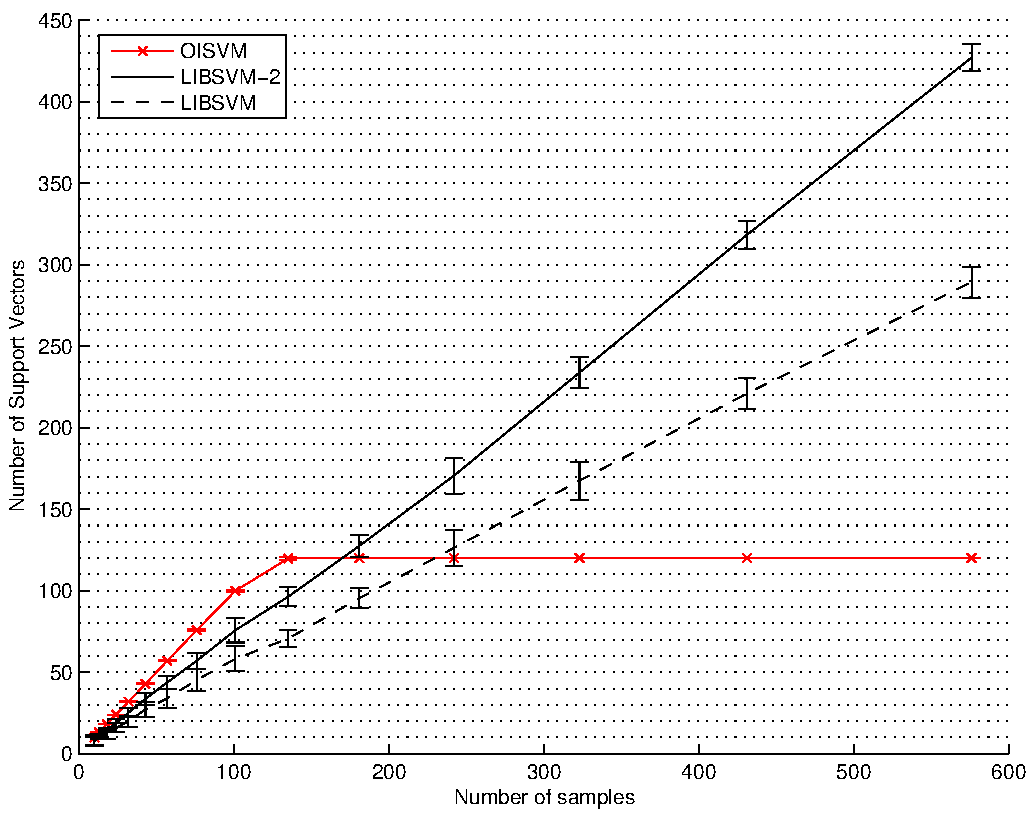
\includegraphics[width=0.47\linewidth]{figs/results/finite_kernel.pdf} &
  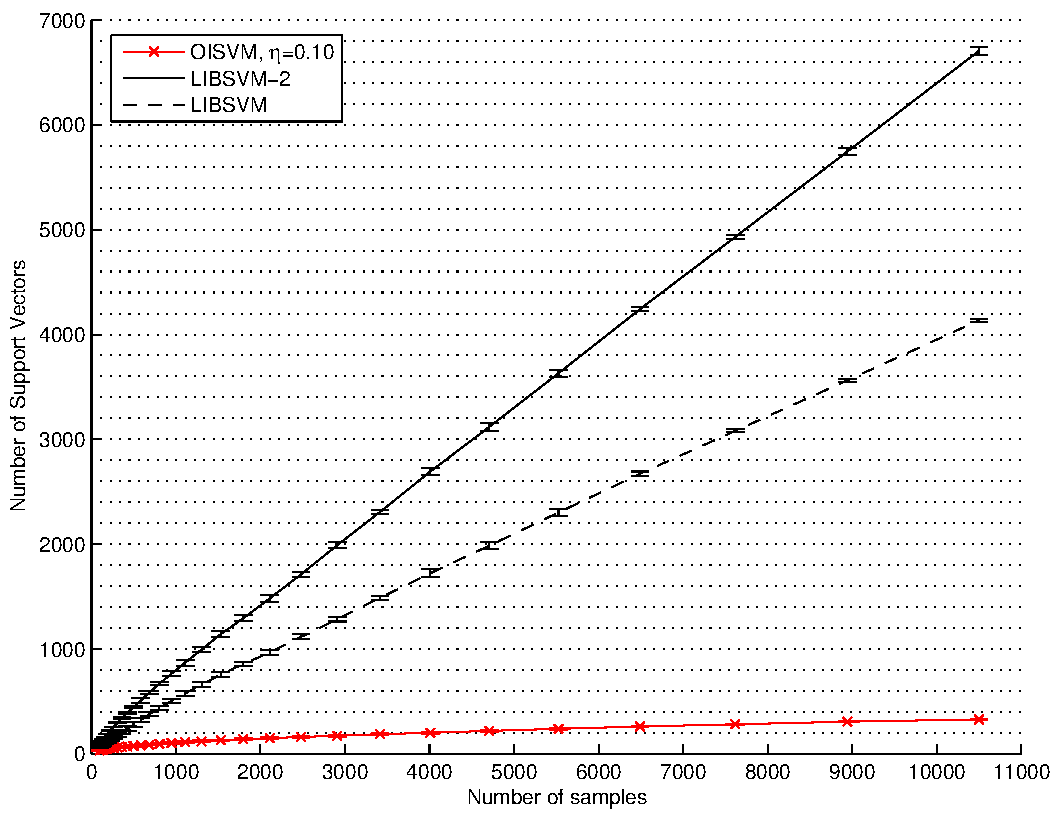
\includegraphics[width=0.47\linewidth]{figs/results/adult7.pdf}
  \end{tabular}
  \caption{Comparison of OISVM and LIBSVM on the \emph{Diabetes}
  (left pane) and \emph{Adult7} (right pane) benchmarks. Diabetes is
  solved using a polynomial kernel with degree $3$, while Adult7 is
  solved using a Gaussian kernel.}
\label{fig:ad7}
\end{figure*}

\begin{table*}
\begin{center}
\begin{tabular}[!h]{|l|c|c|c|}
\hline
  Benchmark & Class. rate    & \% SVs          & \% SVs        \\
       name & loss           & vs. LIBSVM-2    & vs. LIBSVM    \\ \hline
     Breast & $0.47\pm0.82$  & $10.2\pm0.87$   & $22.1\pm1.77$ \\
   Diabetes & $-0.52\pm2.1$  & $40.2\pm2.1$    & $55.2\pm2.73$ \\
   German   & $0.40\pm1.15$  & $6.1\pm0.23$    & $9.2\pm0.35$  \\
   Heart    & $-0.45\pm1.01$ & $10.3\pm0.56$   & $15.5\pm0.94$ \\ \hline
\end{tabular}
\end{center}
\label{table:t1}
\caption{Comparison of OISVM and LIBSVM on more standard benchmarks, solved
 using a Gaussian kernel. For each benchmark, we report the difference
 in classification rate with respect to LIBSVM-2 and the
 percentage of the number of SVs with respect to LIBSVM and
 LIBSVM-2. The value of $\eta$ has been chosen in order not to loose
 more than $0.5\%$ accuracy.}
\end{table*}

Consider Figure \ref{fig:ad7}, left pane: when all samples have been
loaded, LIBSVM-2 has about $427$ SVs, and LIBSVM about $290$. The
kernel used is polynomial with degree $3$ and the benchmark has $8$
features, therefore the dimension of the feature space is
$\binom{10}{3} = 120$ (see, e.g., \cite{Burges98}); and, as expected,
OISVM stops acquiring new SVs when there are exactly $120$, although
it loads a few more before reaching the limit, with respect to the
other approaches. The accuracy (not displayed) is exactly the
same. Again, notice that, after having acquired $120$ SVs, OISVM will
never acquire any more ever, while keeping the same accuracy, whereas
the LIBSVMs do, as theoretically proved in \cite{Steinwart03}.

Consider now Figure \ref{fig:ad7}, right pane: the kernel used is
Gaussian and its dimension is infinite. The benchmark is relevantly
large ($16100$ samples) and complex ($123$ features). Nevertheless,
with an $\eta$ as small as $0.1$, at the end OISVM has less than $5\%$
of the SVs used by LIBSVM-2 and less than $8\%$ with respect to
LIBSVM. The accuracy is $0.063\%\pm0.14$ worse than that of LIBSVM-2.

Lastly, consider Table \ref{table:t1}, which shows the very same data
in compact form for $4$ more standard databases. OISVM attains a
number of SVs which is about $6\%$ to slightly more than $55\%$ of
LIBSVM, whereas the accuracy is basically the same, being slightly
better than LIBSVM in two cases (\emph{Diabetes}, this time solved via
a Gaussian kernel, and \emph{Heart}).

\subsection{Experiments with Real-world Application}
\label{exp:idol2}

We performed a second series of experiments, namely place recognition
in an indoor environment, to evaluate our algorithm. We considered a
realistic scenario where the algorithm had to incrementally update the
model, so to adapt to the variations in an indoor environment due
to human activities over long time spans. These variations include
people appearing in different rooms during working time, objects such
as cups moved or taken in/out of the drawers, pieces of furniture
pushed around, and so forth.   

\begin{figure*}[t]
\centering \footnotesize
\begin{tabular}{@{}c@{\hspace{0.002\linewidth}}c@{\hspace{0.002\linewidth}}c@{\hspace{0.002\linewidth}}c@{\hspace{0.002\linewidth}}c@{\hspace{0.002\linewidth}}c@{\hspace{0.002\linewidth}}c@{\hspace{0.002\linewidth}}c@{}}
% -------------------------------------------------------------------
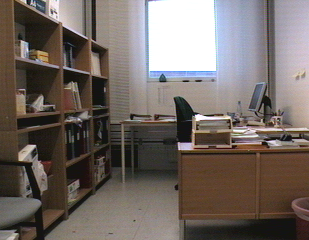
\includegraphics[width=0.123\linewidth]{figs/idol/bo_cloudy.png} &
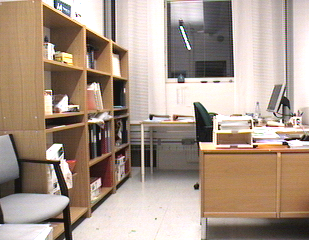
\includegraphics[width=0.123\linewidth]{figs/idol/bo_night.png}  &
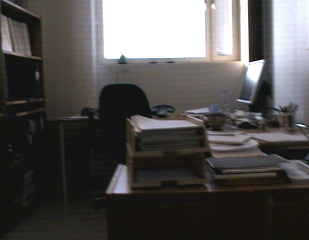
\includegraphics[width=0.123\linewidth]{figs/idol/bo_sunny.png}  &
\includegraphics[width=0.123\linewidth]{figs/idol/cr_cloudy.png} &
\includegraphics[width=0.123\linewidth]{figs/idol/cr_night.png}  &
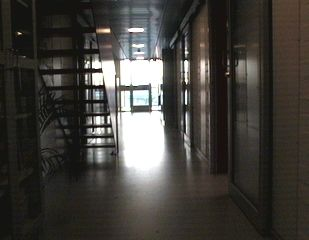
\includegraphics[width=0.123\linewidth]{figs/idol/cr_sunny.png} &
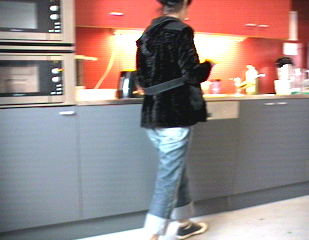
\includegraphics[width=0.123\linewidth]{figs/idol/people1.png}  &
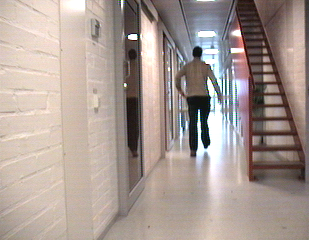
\includegraphics[width=0.123\linewidth]{figs/idol/people2.png}  \\

% -------------------------------------------------------------------
\includegraphics[width=0.123\linewidth]{figs/idol/cup1.png}   &
\includegraphics[width=0.123\linewidth]{figs/idol/cup3.png}   &
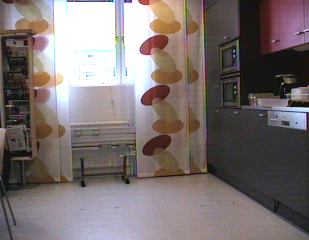
\includegraphics[width=0.123\linewidth]{figs/idol/chair1.png}   &
\includegraphics[width=0.123\linewidth]{figs/idol/chair3.png} &
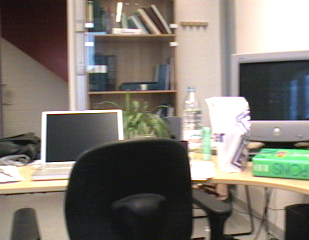
\includegraphics[width=0.123\linewidth]{figs/idol/time1.png} &
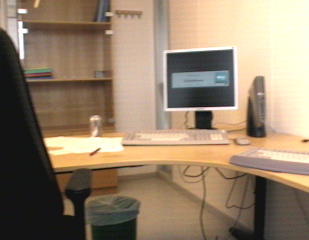
\includegraphics[width=0.123\linewidth]{figs/idol/time2.png} &
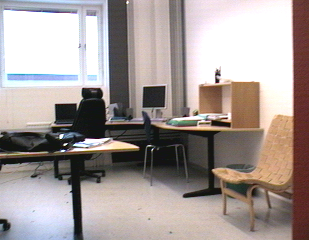
\includegraphics[width=0.123\linewidth]{figs/idol/time3.png}  &
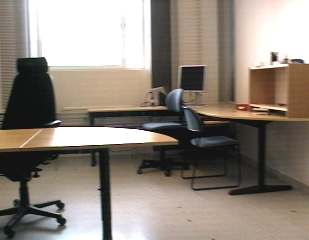
\includegraphics[width=0.123\linewidth]{figs/idol/time4.png}  \\
% -------------------------------------------------------------------

\includegraphics[width=0.123\linewidth]{figs/idol/drive1.png}   &

\includegraphics[width=0.123\linewidth]{figs/idol/drive2.png}   &

\includegraphics[width=0.123\linewidth]{figs/idol/drive3.png}   &
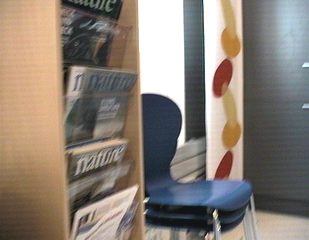
\includegraphics[width=0.123\linewidth]{figs/idol/drive4.png} &
\includegraphics[width=0.123\linewidth]{figs/idol/drive5.png} &
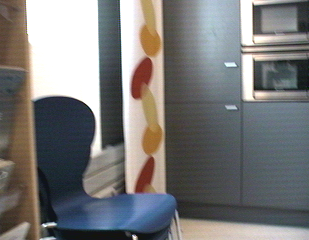
\includegraphics[width=0.123\linewidth]{figs/idol/drive6.png} &
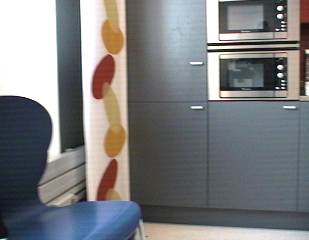
\includegraphics[width=0.123\linewidth]{figs/idol/drive7.png}  &
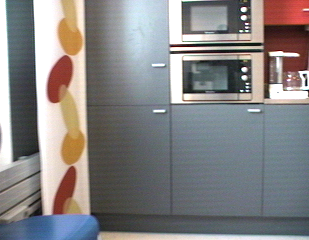
\includegraphics[width=0.123\linewidth]{figs/idol/drive8.png}   \\
% -------------------------------------------------------------------
\end{tabular}
\caption{Sample images illustrating the variations captured in the IDOL2 database.
Images in the top row show the variability introduced by changes in illumination
for two rooms (first six images) as well as people appearing in the environment.
The middle row shows the influence of people's everyday activity (first four images)
as well as larger variations which happened over a time span of 6 months. Finally, the
bottom row illustrates the changes in viewpoint observed for a series of images acquired 
one after another in 1.6 second.}
\label{fig:idol}
\end{figure*}

Experiments were conducted on  a newly introduced database called IDOL2 
(Image Database for rObot Localization 2, \cite{luo:idol2}), 
which contains 24 image sequences acquired using a perspective
camera mounted on two mobile robot platforms. The acquisition was
performed within an indoor laboratory environment consisting of five 
rooms of different functionality. The sequences were acquired under
various weather and illumination conditions (sunny, cloudy, and night)
and across a time span of six months. Thus, this data capture natural
variability that occurs in real-world environments because of both 
natural changes in the illumination and human activity. Fig. \ref{fig:idol} 
shows some sample images from the database, illustrating the difficulties of
the task.
The image sequences in the database are divided as follows: for each robot
platform and for each type of illumination conditions, there were
four sequences recorded. Of these four sequences, the first two were 
acquired six months before the last two. This means that, for each robot
and for every illumination condition, there are always two sequences
acquired under similar conditions, and two sequences acquired under very
different conditions. This makes the database suitable for different kinds of
evaluation on the adaptability of an incremental algorithm. For further
details about the database, we refer the readers to \cite{luo:idol2}.

The evaluation was performed using composed receptive field histograms (CRFH)
\cite{linde:icpr04} as global image features and SIFT \cite{lowe99object} for
extracting local features. In the experiments, we consider both $\chi^2$ kernel
for SVM (when use CRFH), and local kernels \cite{wallraven:iccv03} (SIFT).
Similarly to the previous set of experiments, we run the OISVM using different
values of $\eta$, for both kernels.

We benchmarked  OISVM against two approximate incremental SVM extensions: the
standard fixed-partition technique \cite{syed99incremental} and the memory-controlled
incremental SVM \cite{luo:icra07}, a recently introduced version of incremental
SVM, inspired by the work of Downs et~al. \cite{DownsGM01}. We used a similar
experimental method as the one presented in \cite{luo:icra07}. The algorithm was
trained incrementally on three sequences from IDOL2, acquired under similar
illumination conditions with the same robot platform; the fourth sequence was
used for testing. In order to test the various properties of interest of the
incremental algorithms, we need a reasonable number of incremental steps.
Thus, every sequence was splitted into 5 subsequences, so that each subset 
contained one of the five images acquired by the robot every second (image
sequences were acquired at a rate of 5fps). Since during acquisition the camera's
viewpoint continuously changes \cite{luo:icra07}, the subsequences could be
considered as recorded separately in a static environment but for varying pose.
This setup allows us to examine how the algorithms perform on data with less
variations. In order to get a feeling of the variations of the frame images in a
sequence, bottom row of Fig. \ref{fig:idol} shows some sample images acquired
within a time span of 1.6 sec. This setup allows us to examine how the algorithms
perform on data with less variations. As a result, training on each sequence was
performed in 5 steps, using one subsequence at a time, resulting in 15 steps in 
total. Overall, we considered 36 different permutations of training and test
sequences for $chi^2$ kernel and 12 permutations for local kernel 
\footnote{Upon acceptance of the paper, we will report results
on 36 permutations for the local kernel as well (experiments currently running).}; 
here we report average results with standard deviation. 
Fig. \ref{fig:exp:idol}, left, shows the recognition rates of $chi^2$ kernel (top)
and local kernel (bottom) experiments obtained at each step using OISVM and the
other approximate incremental algorithms. Fig. \ref{fig:exp:idol}, right, reports
the number of support vectors stored in the model at each step of the incremental
procedure, for both kernel types.

We see that, performance-wise, all methods achieves statistically comparable results; this
is true for both kernel types. Regarding the growth of the SV solution as the incremental
steps grow, the OISVM algorithm shows a considerable advantage with respect to the fixed partition
and the memory controlled incremental methods. In the case of the $\chi^{2}$
kernel this advantage is truly impressive (Fig \ref{fig:exp:idol}, top right): for $\eta=0.017$ 
and 0.025 the reduction in the number of stored SV is of 34\%/21\% (final incremental step) 
and compared to the fixed-partition method, and of 55\%/36\% (final incremental step) with
respect to the memory-controlled algorithm. Even more important, OISVM, for these two 
values of $\eta$, has found a plateau in memory, while for the other two methods
the trend seems to be of a growth (less pronounced for the memory controlled algorithm,
which plot might be interpreted as an asyntotic plateau) proportional to 
the number of training data. Note that the choice of the parameter $\eta$ is crucial for
achieving an optimal trade-off between compactness of the solution and optimal performance.  

It is very interesting to note that, in the case of the local kernel, the memory reduction
for OISVM is less pronounced with respect to the memory-controlled method, and there isn't a clear 
plateau in memory growth by any of the algorithms. A possible explanation
might be that the local kernel is not a Mercer kernel, and thus the solution is never guaranteed to 
be optimal \textbf{fixme: does anybody anything to say more/better about this?}.

We can conclude that these results are in agreement with those obtained on the
machine learning benchmark databases, and show the effectiveness of OISVM in
controlling the growth of the SV solution for online learning scenarios.



\begin{figure*}[t]
  \centering \footnotesize
  \begin{tabular}{c@{\hspace{0.5cm}}c}
  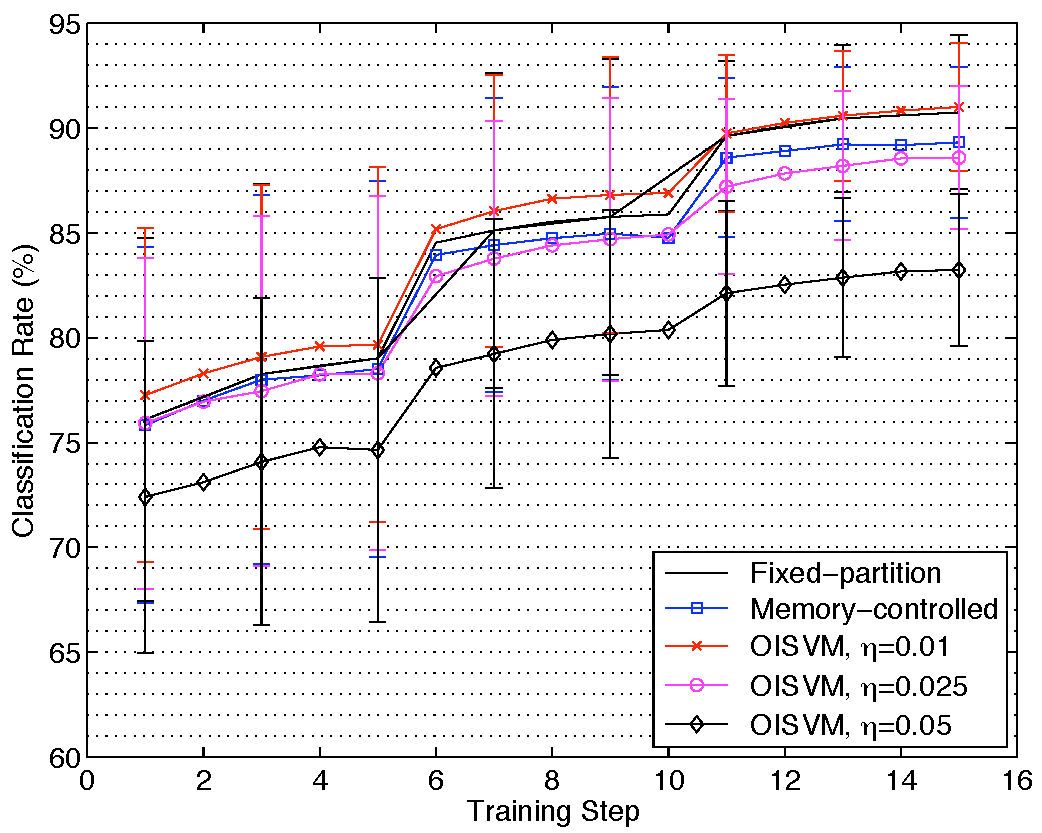
\includegraphics[width=0.47\linewidth]{figs/results/chi_cr} &
  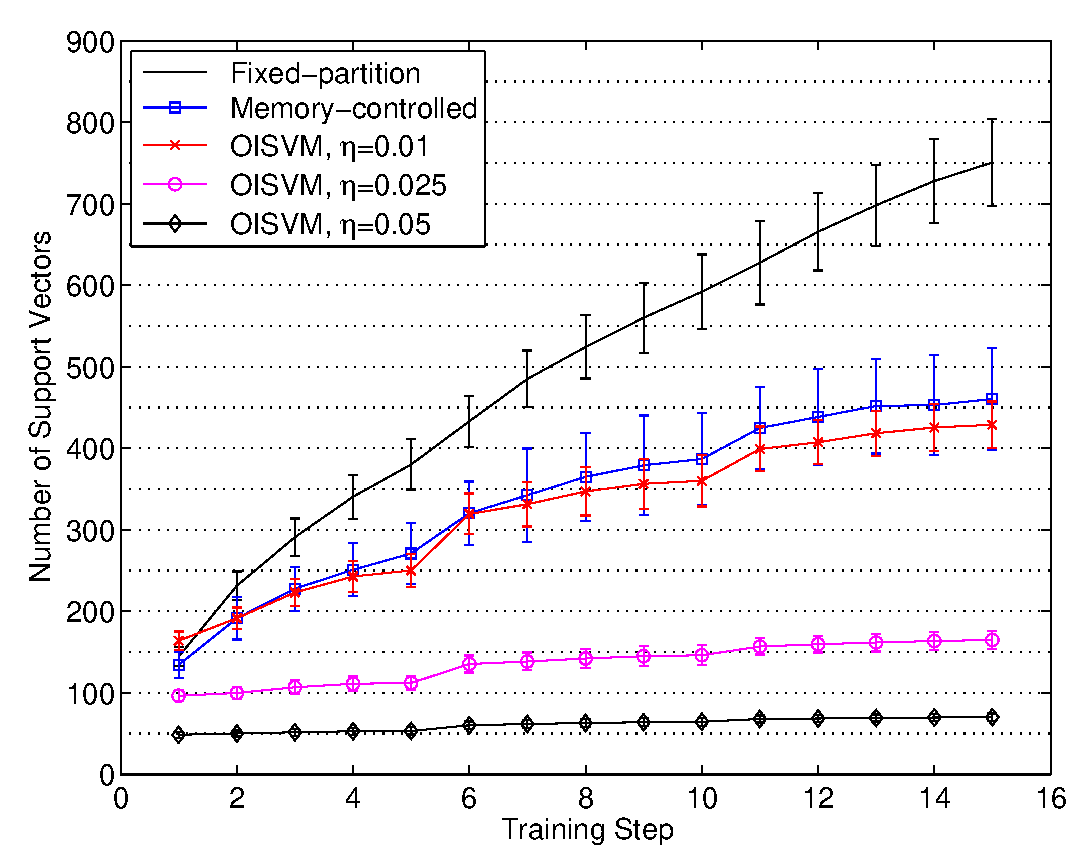
\includegraphics[width=0.47\linewidth]{figs/results/chi_sv} \vspace{0.1cm}\\
  \multicolumn{2}{c}{(a)~Number of support vectors and classification rate obtained at each incremental step using $chi^2$ kernel.}  \\
  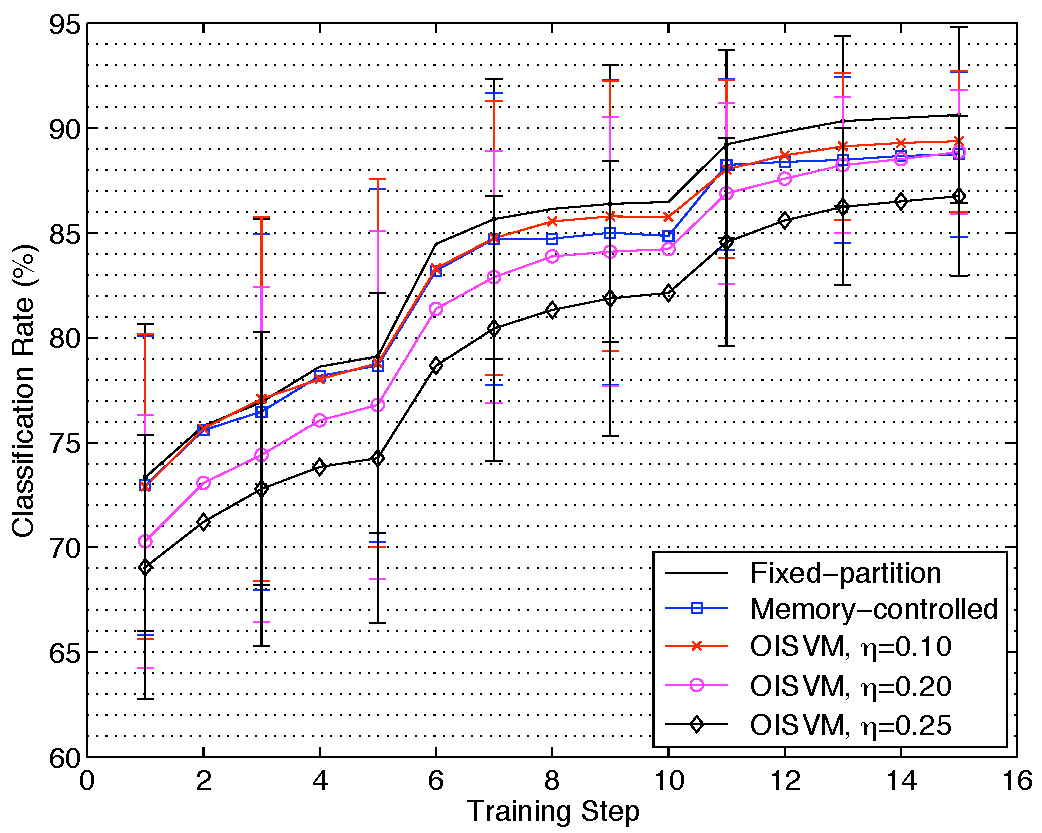
\includegraphics[width=0.47\linewidth]{figs/results/local_cr} &
  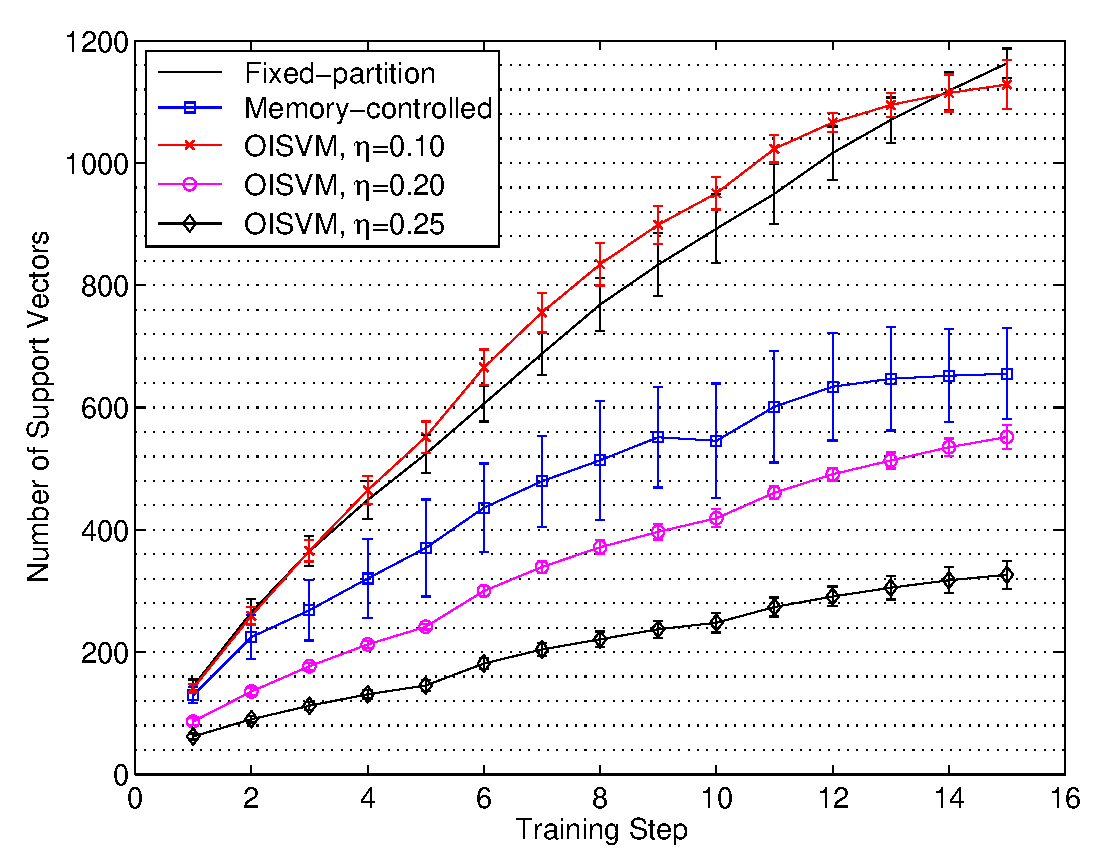
\includegraphics[width=0.47\linewidth]{figs/results/local_sv} \vspace{0.1cm}\\
  \multicolumn{2}{c}{(b)~Number of support vectors and classification rate obtained at each incremental step using local kernel.} \\
  \end{tabular}
\caption{Average results obtained for experiment performed on the IDOL2 database, using
         OISVM with  three different values of $\eta$, the 
         fixed-partition and memory-controlled methods. }
\label{fig:exp:idol}
\end{figure*}


\section{Conclusions}
\label{sec:concl}
In this paper we have shown a promising improvement to Support Vector
Machines, that we call Online Independent Support Vector Machines
(OISVM). OISVMs can effectively solve the problem of place recognition
by a mobile robot, at least in the experiment we have shown. OISVMs
were tested on the IDOL2 image database, which consists of image
sequences acquired by robot platforms under different weather
conditions and across a time span of several months; that is, in
various lighting conditions and object placements, and acquired by two
different robot platforms. OISVMs avoid using in the solution those
support vectors which are linearly dependent of previous ones in the
feature space. The optimization problem is solved via an incremental
algorithm which benefits of the small number of the basis vectors.

As far as we know, this method is different from all
analogous procedures presented so far in literature (e.g.,
\cite{DownsGM01,nguyen2005,LeeM01,schoel06,KeerthiCDC06}) since it
is \emph{not} an after-training simplification and it assumes
\emph{no knowledge whatsoever} of the full training set beforehand.
Moreover in case of finite-dimensional kernel and $\eta=0$, the
solution is exactly the same of the standard formulation because
there is any approximation is used.

Our experimental results show that in
the case of infinite-dimensional kernels, the number of support vectors
is dramatically reduced at the price of a negligible degradation in
the accuracy. In fact in the case of $\chi^2$ kernel, we get as few
as $3.5$ times less SVs respect to the batch formulation and $3$
times less respect to the fixed-partition method, while retaining
essentially the same accuracy. In the case of the local kernel...
[\textbf{COMPLETE AFTER WE HAVE THE FINAL RESULTS}]

Since the training and testing time depend polynomially on the
number of support vectors, reducing them bring an obvious speed up. A
careful study of the relationship between $\eta$ and the degradation
in performance is being carried on; in fact, according to
\cite{engel2004}, imposing a value of $\eta$ strictly larger than zero
will eventually result in a \emph{finite} number of basis vectors,
\emph{even in the case the feature space is
infinite-dimensional}. On going research is on finding a precise
relationship between $\eta$ and this number to allow
us to precisely dimension the machine depending on the required
precision.

% ------------------------------------------------------------------------ 

{\small
\bibliographystyle{ieee}
\bibliography{cvpr2007}
}

\end{document}
